\documentclass[a4paper]{article}
\usepackage{amsfonts}
\usepackage{amsmath}
\usepackage{amssymb}
\usepackage{graphicx}

\newcommand{\dint}{\displaystyle\int}

\begin{document}

\noindent \large Auteur: Rob Willemsen \\
\noindent \large Studierichting: Informatica \\
\noindent \large Oefeningenreeks 5G nr. 16.4 \\

\medskip

\normalsize

$a=1$ en $b=27$ en $r=y^{\tfrac{1}{3}}-1$ \\

$V = \pi \dint _1^{27} (y^{\tfrac{1}{3}}-1)^2 dy$ \\

$= \pi \dint _1^{27} (y^{\tfrac{2}{3}} - 2y^{\tfrac{1}{3}} + 1) dy$ \\

$= \pi \left[ \dfrac{3}{5}y^{\tfrac{5}{3}} - \dfrac{3}{2}y^{\tfrac{4}{3}} + y \right]_1^{27}$ \\

$= \pi \left( \dfrac{3}{5}27^{\tfrac{5}{3}} - \dfrac{3}{2} \cdot 27^{\tfrac{4}{3}} + 27 \right) - \pi \left( \dfrac{3}{5}1^{\tfrac{5}{3}} - \dfrac{3}{2} \cdot 1^{\tfrac{4}{3}} + 1 \right)$ \\

$= \pi \left( \dfrac{729}{5} - \dfrac{243}{2} + 27 \right) - \pi \left( \dfrac{3}{5} - \dfrac{3}{2} + 1 \right)$ \\

$= \pi \left( \dfrac{513}{10} - \dfrac{1}{10}\right)$ \\

$= \dfrac{512\pi}{10}$ \\

$= \dfrac{256\pi}{5}$ \\

\begin{figure}[h]
\centering
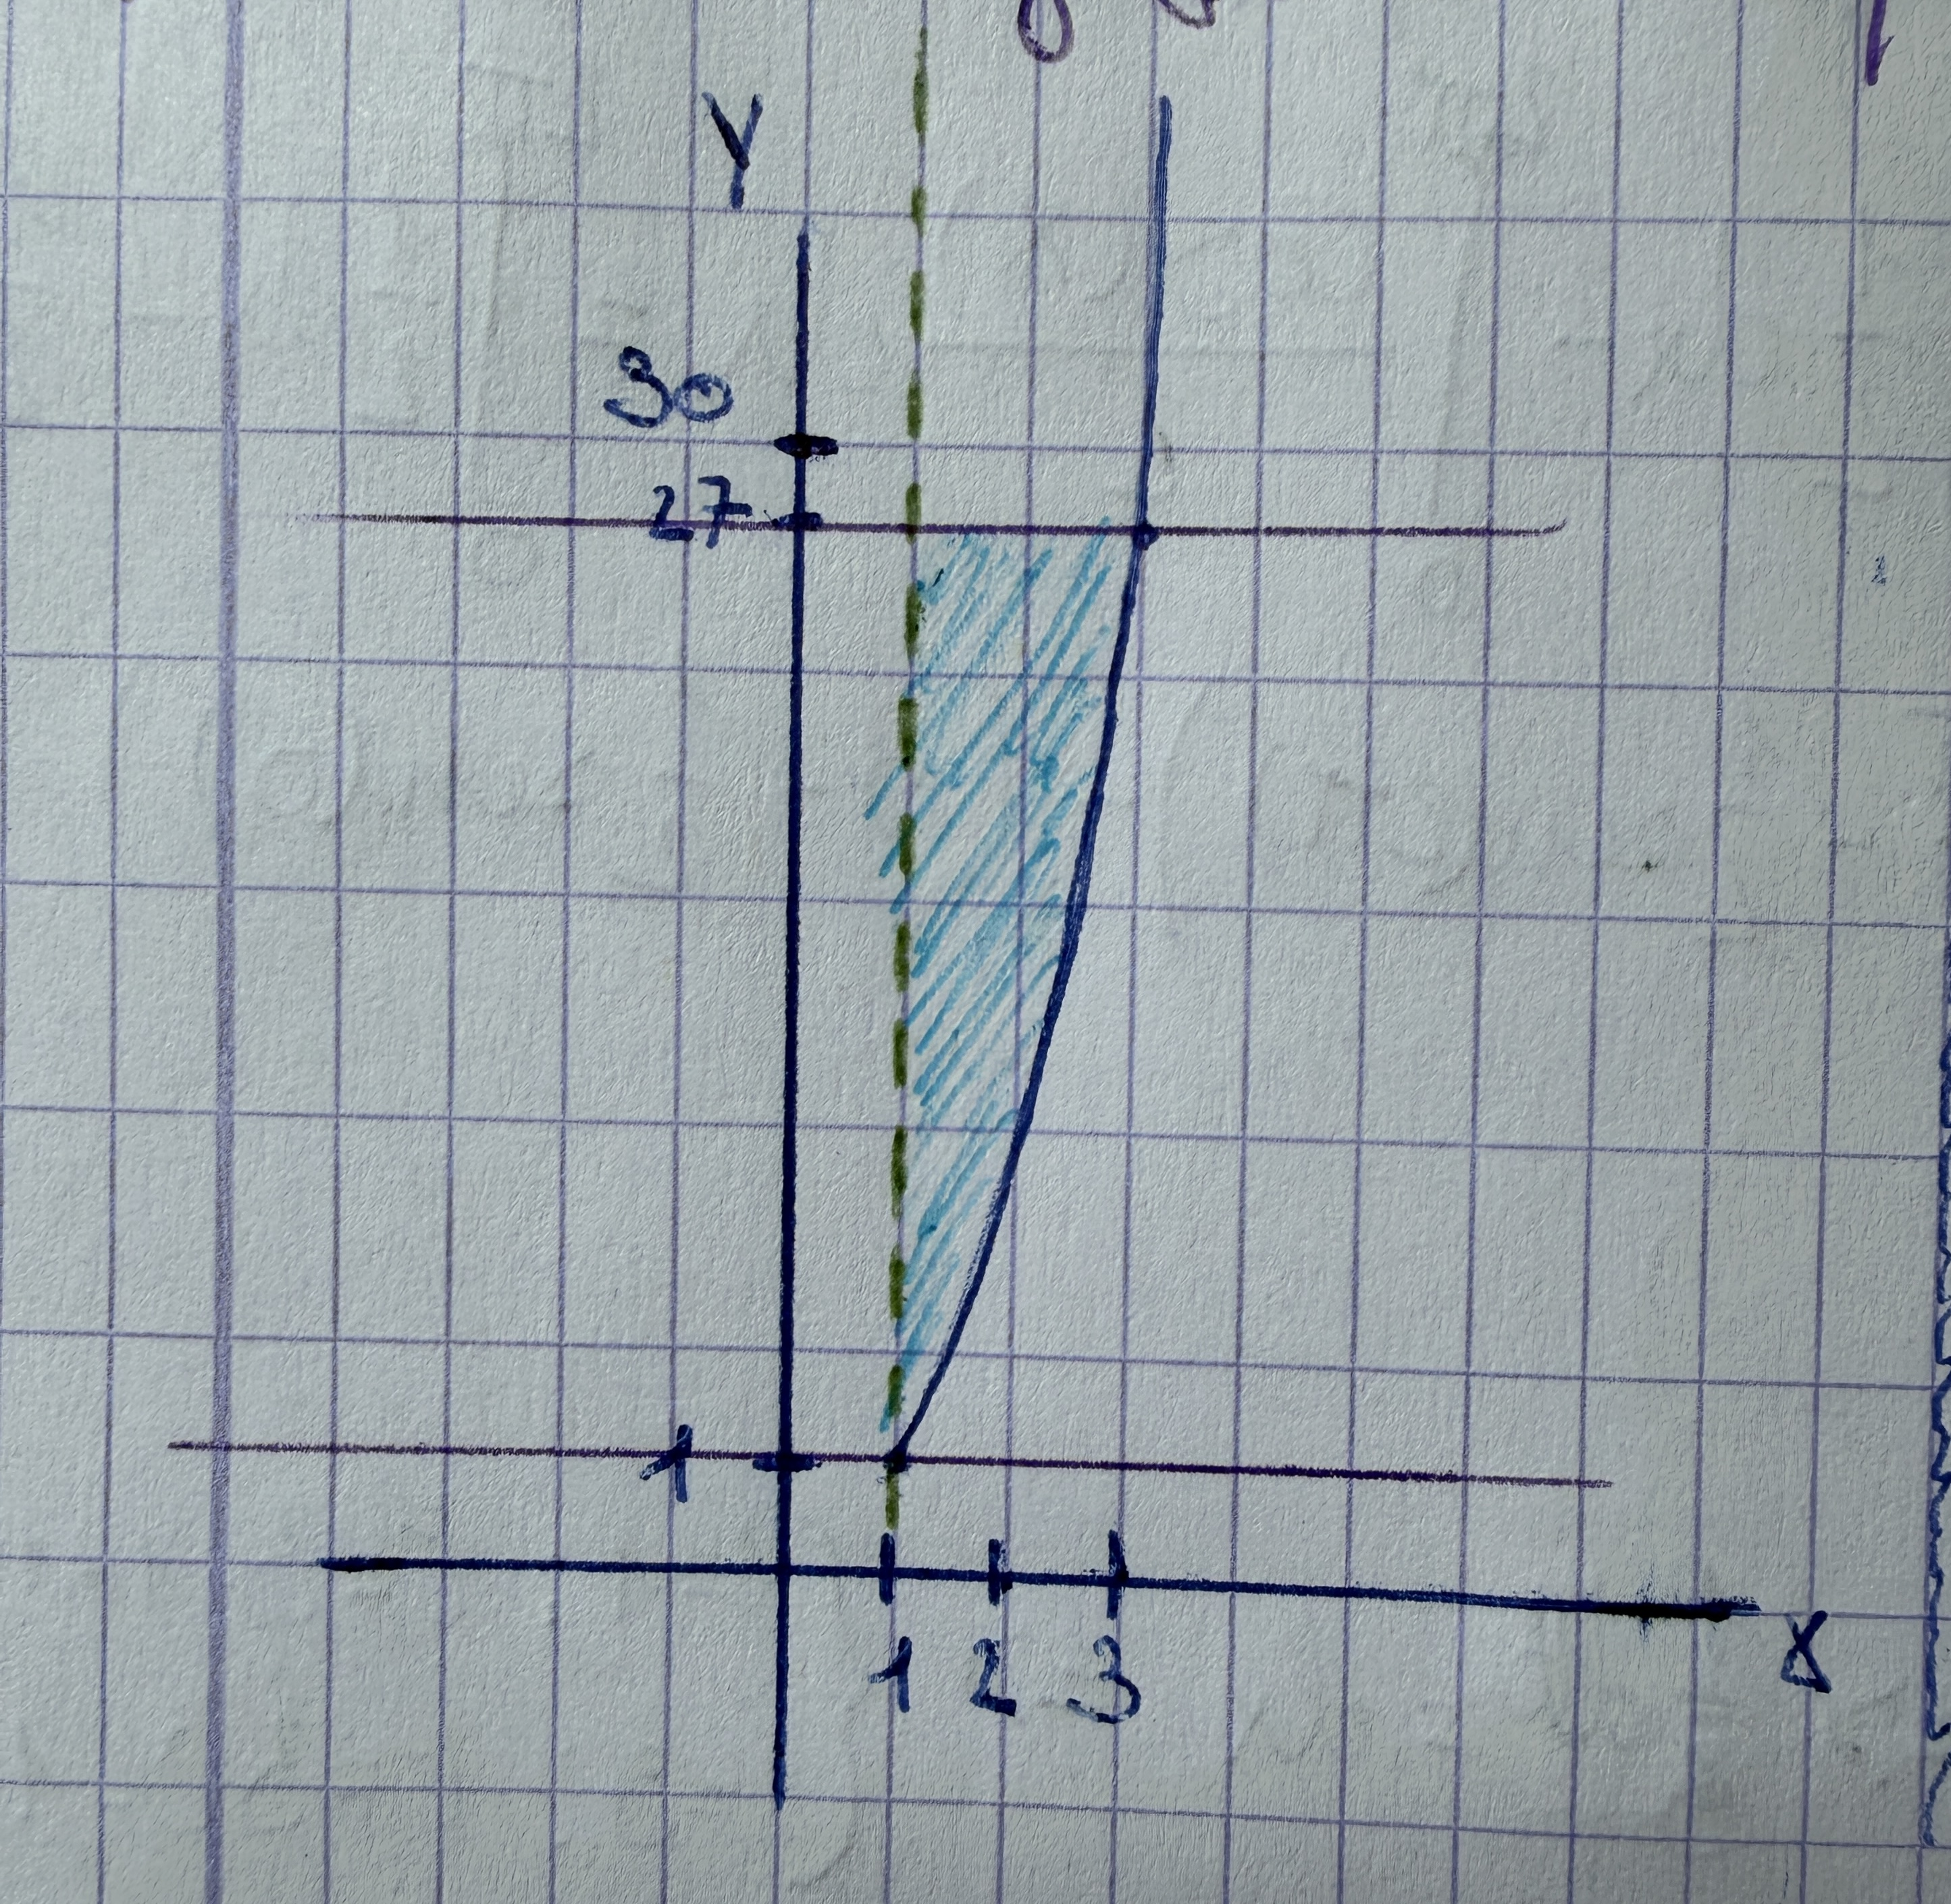
\includegraphics[width=0.5\linewidth]{5G-16.4-rob.willemsen.INF.png}
\end{figure}

\begin{thebibliography}{999}
%\bibitem{a} Referentie
\end{thebibliography}
\end{document}